\documentclass[10pt]{article}
\usepackage{amsmath}
\usepackage{graphics}
\usepackage{graphicx}
\usepackage{float}

\addtolength{\oddsidemargin}{-.875in}
	\addtolength{\evensidemargin}{-.875in}
	\addtolength{\textwidth}{1.75in}

	\addtolength{\topmargin}{-.875in}
	\addtolength{\textheight}{1.75in}
\renewcommand{\baselinestretch}{0.97}
\title{COL 774: Machine Learning Assignment 1}
\author {Saurabh Godse [2018MCS2019]}

\date{Due date: February 12, 2019, 11:59pm IST}

\begin{document}

\maketitle

\section{Gradient Descent}

\begin{itemize}
 \item Learning Rate: 0.01.
 \item Value of $\theta_0$ and $\theta_1$ are [0.9963085  0.00133978] respectively.
 \item The Stopping Criteria is the difference in the cost function of $10 ^ {-9} $.
\end{itemize}

\begin{table}[h!]
	\centering
	\begin{tabular}{||c|c|c|c||} 
 	\hline
 	LearningRate & TotalIterations & Overshoots & Converges \\ [0.5ex] 
 	\hline
 	0.1  & 89 & No & Yes \\ 
 	0.5 & 16 & No & Yes \\
 	0.9 & 6 & No & Yes \\
 	1.3 & 10 & Yes & Yes \\
 	1.7 & 29 & Yes & Yes \\ 
 	2.1 & Nan & Yes & No \\
 	2.5 & Nan & Yes & No \\ [1ex]
 	\hline
	\end{tabular}

	\caption{Learning Rates and Observation}
	\label{table:1}
\end{table}

\begin{figure}[H]
	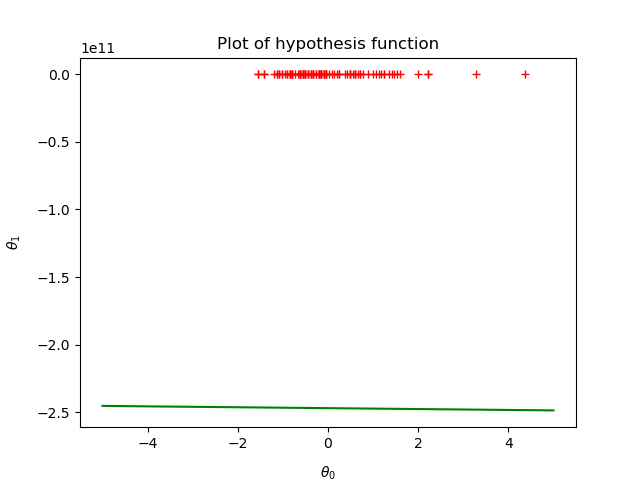
\includegraphics[width = 15cm,height = 10cm]{Q1_b}
	\caption{Gradient Descent}
\end{figure}

\begin{figure}[H]
	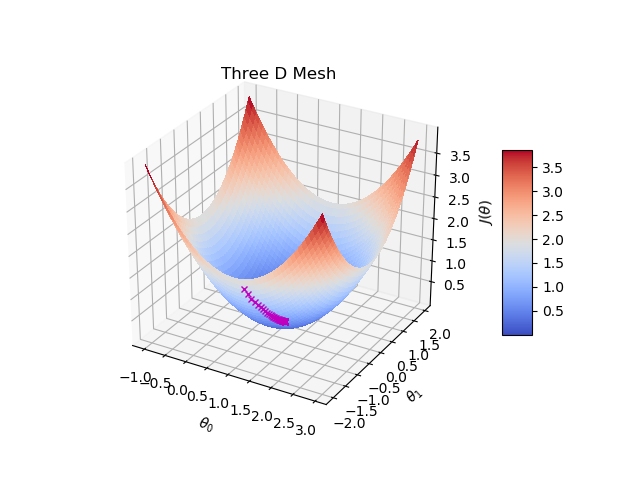
\includegraphics[width = 15cm,height = 10cm]{Q1_c}
	\caption{3d mesh plot of Costfunction}
\end{figure}

%\begin{figure}[H]
%	\includegraphics[width = 15cm,height = 10cm]{gradcon}
%	\caption{3d mesh plot of Costfunction}
%\end{figure}

\begin{figure}[H]
	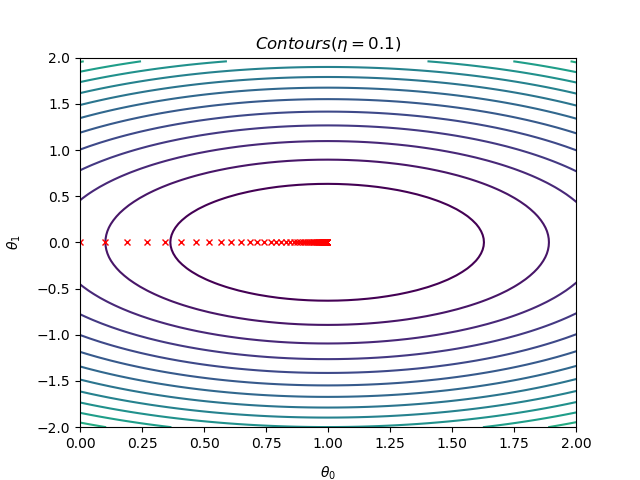
\includegraphics[width = 15cm,height = 10cm]{Q1_d01}
	\caption{Contour at eta = 0.1}
\end{figure}

\begin{figure}[H]
	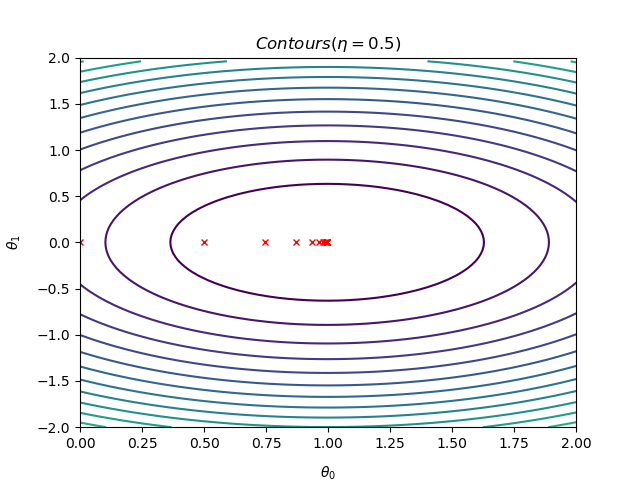
\includegraphics[width = 15cm,height = 10cm]{Q1_d05}
	\caption{Contour at eta = 0.5}
\end{figure}

\begin{figure}[H]
	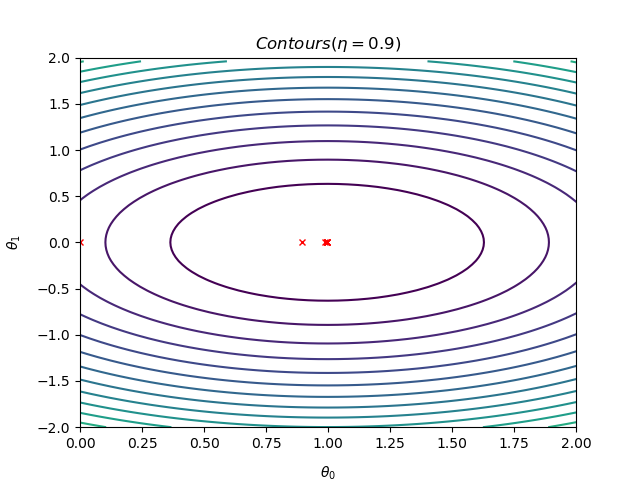
\includegraphics[width = 15cm,height = 10cm]{Q1_d09}
	\caption{Contour at eta = 0.9}
\end{figure}

\begin{figure}[H]
	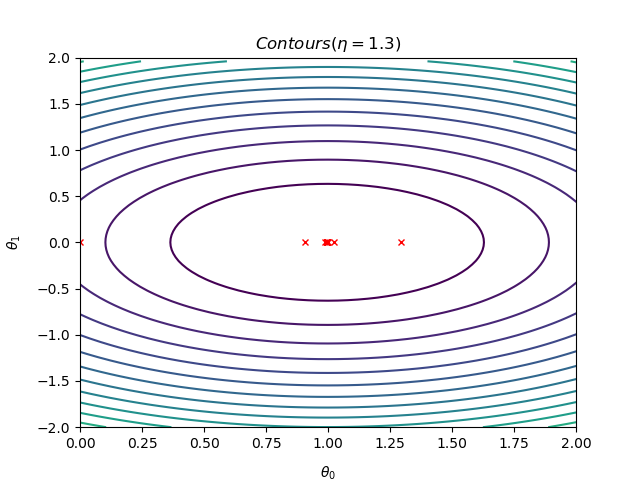
\includegraphics[width = 15cm,height = 10cm]{Q1_d13}
	\caption{Contour at eta = 1.3}
\end{figure}

\begin{figure}[H]
	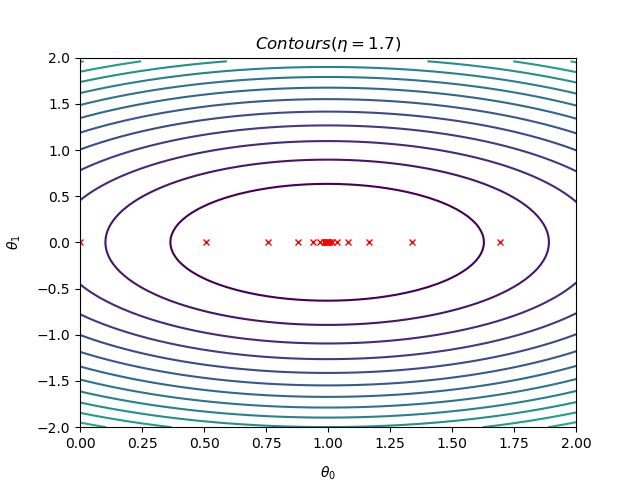
\includegraphics[width = 15cm,height = 10cm]{Q1_d17}
	\caption{Contour at eta = 1.7}
\end{figure}

\section{Locally Weighted Linear Regression}
%%% Fill in your content here.


\[J(\theta) = \frac{1}{2m} (X\theta - Y)^TW(X\theta -Y)\]

\[On \ solving \ for \ \frac{dJ{(\theta)}}{d\theta} = 0, \ we \ get \ \theta = (X^TWX)^{-1}X^TWY\]

\begin{itemize}
 \item Best Value of tau should be 0.3 because it generalizes the data well.
 \item Larger the value of tau it underfits the data or produces a linear fit to the data.
 \item Smaller value of tau will lead to overfitting issues.
\end{itemize}

\begin{figure}[H]
	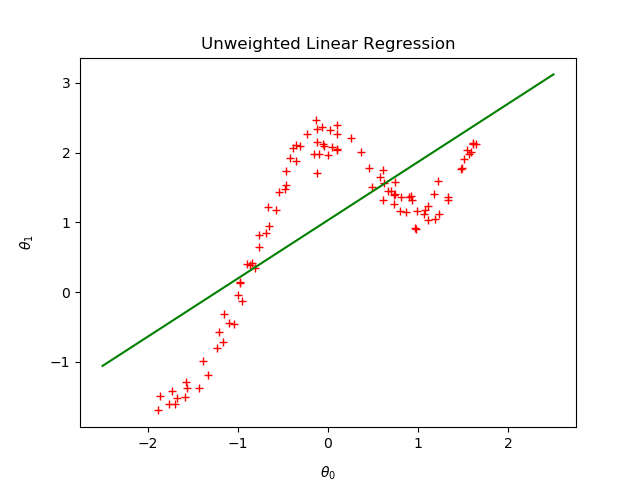
\includegraphics[width = 15cm,height = 10cm]{Q2_a}
	\caption{Analytical Solution}
\end{figure}

\begin{figure}[H]
	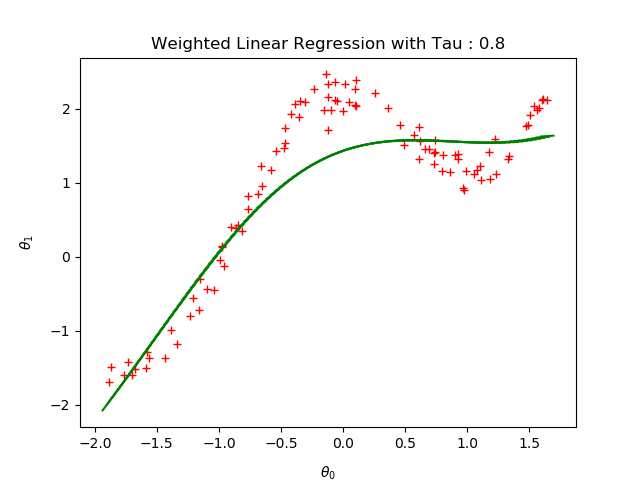
\includegraphics[width = 15cm,height = 10cm]{Q2_b08}
	\caption{Locally Weighted Solution at tau = 0.8}
\end{figure}

\begin{figure}[H]
	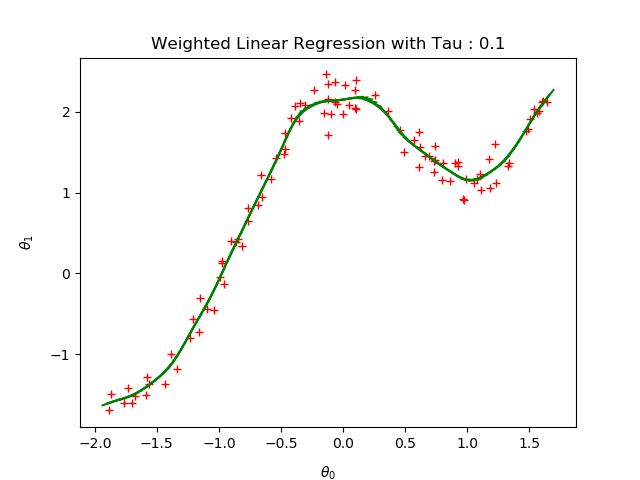
\includegraphics[width = 15cm,height = 10cm]{Q2_b01}
	\caption{Locally Weighted Solution at tau = 0.1}
\end{figure}

\begin{figure}[H]
	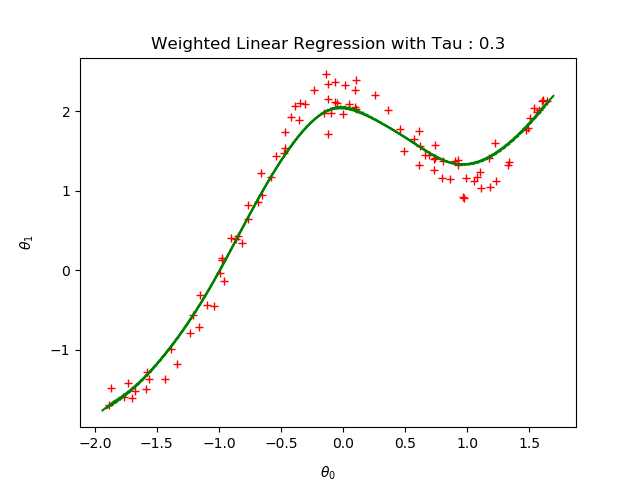
\includegraphics[width = 15cm,height = 10cm]{Q2_b03}
	\caption{Locally Weighted Solution at tau = 0.3}
\end{figure}

\begin{figure}[H]
	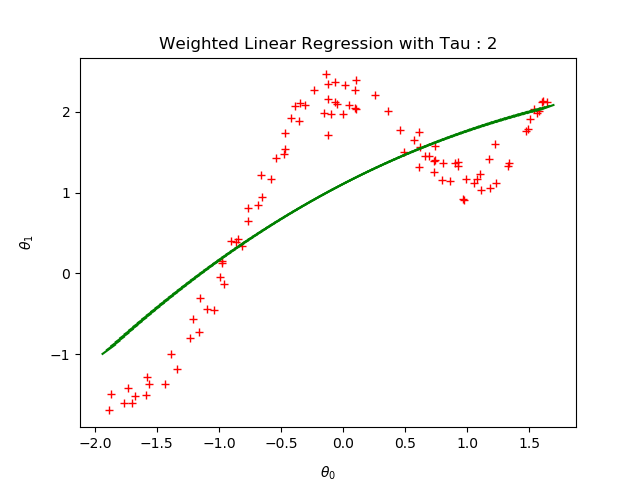
\includegraphics[width = 15cm,height = 10cm]{Q2_b2}
	\caption{Locally Weighted Solution at tau = 2}
\end{figure}

\begin{figure}[H]
	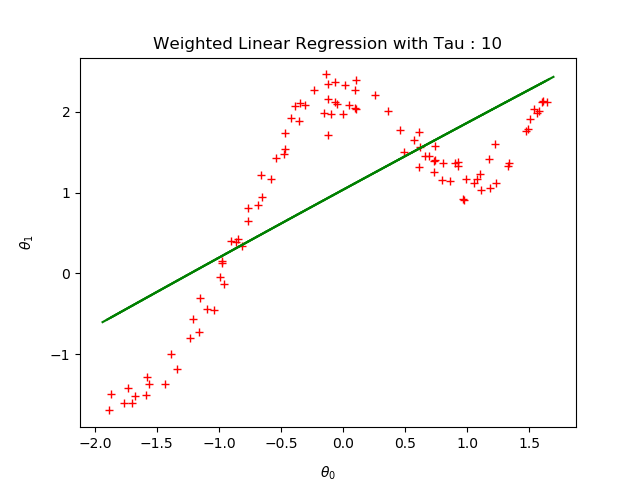
\includegraphics[width = 15cm,height = 10cm]{Q2_b10}
	\caption{Locally Weighted Solution at tau = 10}
\end{figure}
 

\section{Logistic Regression}

\[Hessian = -X^T(g(\theta^TX)(1 - g(\theta^TX))X\]
\[Gradient = X^TY - X^Tg(\theta^TX))\]
\[\text{On Applying Newton's Method we get}\]
\[\theta^{t+1} = \theta^t - \frac{Gradient}{Hessian}\]

\begin{itemize}
\item Value of $\theta_0, \theta_1, \theta_2$ are [ 0.22329537  1.96261552 -1.9648612 ] respectively.
\end{itemize}

\begin{figure}[H]
	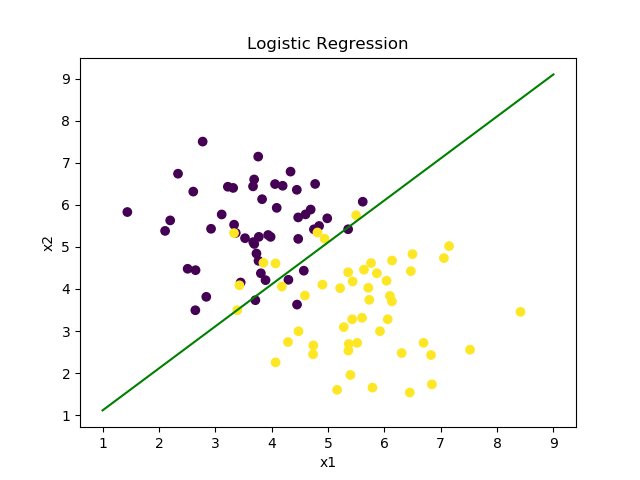
\includegraphics[width = 15cm,height = 10cm]{Q3_b}
	\caption{Logistic Regression with Newton's Method}
\end{figure}


\section{Gaussian Discriminant Analysis}

\subsection{In case of Same Covariance}

\begin{itemize}
\item Covariance \[\Sigma\] \begin{center}
\begin{tabular}{ |c|c|}
\hline
 28748.2 & -2674.8  \\
 \hline 
 -2674.8 & 112325. \\
\hline   
\end{tabular}
\end{center}
\item Mean of Alaska $$\mu_0$$ \begin{center}
\begin{tabular}{ |c|c|}
\hline
 98.38 & 429.66  \\
 \hline        
\end{tabular}
\end{center}
\item Mean of Canada $$\mu_1$$ \begin{center}
\begin{tabular}{ |c|c|}
\hline
 137.46 & 366.62  \\
\hline  
\end{tabular}
\end{center}
\end{itemize}


\subsection{In case of different Covariance}
E0 :  [[ 255.3956 -184.3308]
 [-184.3308 1371.1044]]
E1 :  [[319.5684 130.8348]
 [130.8348 875.3956]]

\begin{itemize}
\item Covariance of Alaska \[\Sigma_0\] \begin{center}
\begin{tabular}{ |c|c|}
\hline
 255.3956 & -184.3308  \\
 \hline 
 -184.3308 & 1371.1044 \\
\hline       
\end{tabular}
\end{center}
\item Covariance of Canada \[\Sigma_1\] \begin{center}
\begin{tabular}{ |c|c|}
\hline
 319.5684 & 130.8348  \\
 \hline 
 130.8348 & 875.3956 \\
\hline       
\end{tabular}
\end{center}
\item Mean of Alaska $$\mu_0$$ \begin{center}
\begin{tabular}{ |c|c|}
\hline
 98.38 & 429.66  \\
 \hline        
\end{tabular}
\end{center}
\item Mean of Canada $$\mu_1$$ \begin{center}
\begin{tabular}{ |c|c|}
\hline
 137.46 & 366.62  \\
\hline       
\end{tabular}
\end{center}
\end{itemize}

\subsection{Equation of the boundary}

$$P(y=1| x;\theta) = P(y=0|x;\theta)$$
$$P(x|y=1;\theta)P(y=1;\phi) = P(x|y=0;\theta)P(y=0;\phi)$$
$$\text{Solving the above equation yields}$$
$$\frac{1}{2}[(X-\mu_1)^T\Sigma_1^{-1}(X-\mu_1) - (X-\mu_0)^T\Sigma_0^{-1}(X-\mu_0)] = log(\frac{\phi}{1-\phi}) - log(\frac{|\Sigma_1|^{\frac{-1}{2}}}{|\Sigma_0|^{\frac{-1}{2}}})$$

$$\Sigma_0 = \Sigma_1 = \Sigma \ \text{Same Covariance}$$
$$\text{We obtain a linear boundary whose equation is given by}$$

$$X^T\Sigma^{-1}\mu_0 - X^T\Sigma^{-1}\mu_1 + \mu_1^T\Sigma^{-1}\mu_1 - \mu_0^T\Sigma^{-1}\mu_0 - log(\frac{\phi}{1-\phi}) = 0$$



$$\Sigma_0 \neq \Sigma_1 \ \text{Different Covariance}$$

$$\text{We obtain a Quadratic boundary whose equation is given by}$$

$$X^T\Sigma_0^{-1}X -X^T\Sigma_1^{-1}X + X^T\Sigma_0^{-1}\mu_0 - X^T\Sigma_1^{-1}\mu_1 + \mu_1^T\Sigma_1^{-1}\mu_1 - \mu_0^T\Sigma_0^{-1}\mu_0 - log(\frac{\phi}{1-\phi}) + log(\frac{|\Sigma_1|^{\frac{-1}{2}}}{|\Sigma_0|^{\frac{-1}{2}}}) = 0$$

\begin{figure}[H]
	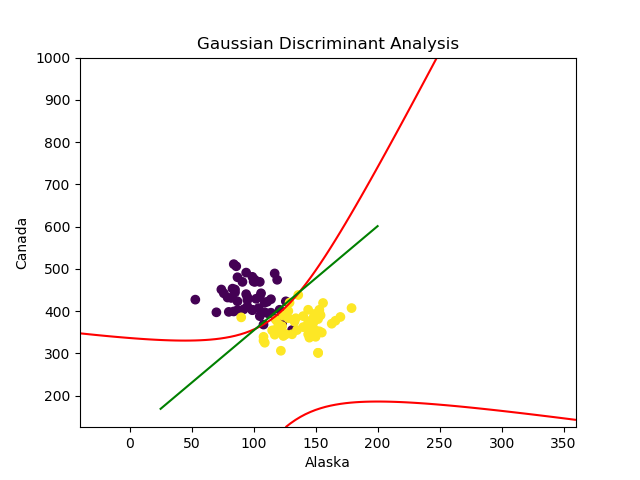
\includegraphics[width = 15cm,height = 10cm]{Q4_e}
	\caption{Gaussain Discriminant Analysis Containing Both Linear and Quadratic Boundary}
\end{figure}
\end{document}